\begin{figure}
    % WARNING: DO NOT CHANGE MANUALLY, CHANGES WILL BE OVERWRITTEN
        \ifdefined\AAAINV\else
        \newcommand\A[2]{\mathbf{A}_{#2}^{#1}}
        \newcommand\B[2]{\mathbf{B}_{#2}^{#1}}
        \newcommand\AINV[2]{(\A{#1}{#2})^{-1}}
        \newcommand\BINV[2]{(\B{#1}{#2})^{-1}}
        \newcommand\AAA[1]{\mathbf{A}^{#1}}
        \newcommand\BBB[1]{\mathbf{B}^{#1}}
        \newcommand\AAAINV[1]{(\AAA{#1})^{-1}}
        \newcommand\BBBINV[1]{(\BBB{#1})^{-1}}
        \newcommand\R{\mathbf{R}}
        \newcommand\RINV{\mathbf{R}^{-1}}
        \newcommand\M{\mathbf{M}}
        \newcommand\El{\ell'}
        \newcommand\MINV{\mathbf{M}^{-1}}
        \newcommand\Min{m_{in}}
        \newcommand\Mout{m_{out}}
        \newcommand\XOR[1]{\mathbf{X}\left[#1\right]}
        \fi
        \ifdefined\aCipher\else
        \newcommand\aCipher{\texttt{Sparkle}}
        \newcommand\FigDef[2]{\caption{#2}\label{#1}}
        \newcommand\PathFig[1]{NON_EXISTANT_PATH/#1}
        \fi
    \caption{Attack on 4.5-step \aCipher{} without whitening.
                            The green dots show known values, the purple crosses show zero differences.
                            The red dashed area highlights the part being attacked, the purple dashed area shows the part with the target differential transition.}
    \label{fig:mitm4.5nowhit}
    \IfFileExists{\PathFig{mitm_4p5steps_nowhitening.pdf}}{
    \includegraphics{\PathFig{mitm_4p5steps_nowhitening.pdf}}
    }{
    \centering
    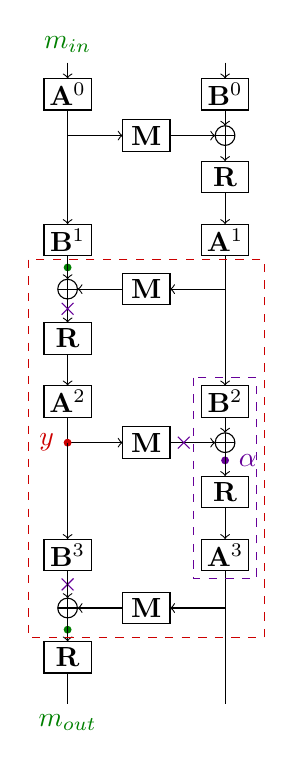
\begin{tikzpicture}[xscale=1.0,yscale=-1.0]
        \draw (0.0,0.0) node[anchor=south,green!50!black] {$\Min$};
        \draw[->] (0.0,0.0) -- (0.0,0.2);
        \draw (-0.3,0.2) rectangle (0.3,0.6) node[pos=0.5] {$\AAA{0}$};
        \draw[->] (2.0,0.0) -- (2.0,0.2);
        \draw (1.7,0.2) rectangle (2.3,0.6) node[pos=0.5] {$\BBB{0}$};
        \draw (0.0,0.6) -- (0.0,0.925);
        \draw[->] (2.0,0.6) -- (2.0,0.8);
        \draw (2.0,0.925) ellipse (0.125 and 0.125);
        \draw (2.0,0.8) -- (2.0,1.05);
        \draw (1.875,0.925) -- (2.125,0.925);
        \draw[->] (0.0,0.925) -- (0.7,0.925);
        \draw (0.7,0.725) rectangle (1.3,1.125) node[pos=0.5] {$\M$};
        \draw[->] (1.3,0.925) -- (1.875,0.925);
        \draw[->] (2.0,1.05) -- (2.0,1.25);
        \draw (1.7,1.25) rectangle (2.3,1.65) node[pos=0.5] {$\R$};
        \draw (0.0,0.925) -- (0.0,1.85);
        \draw (2.0,1.65) -- (2.0,1.85);
        \draw[->] (0.0,1.85) -- (0.0,2.05);
        \draw (-0.3,2.05) rectangle (0.3,2.45) node[pos=0.5] {$\BBB{1}$};
        \draw[->] (2.0,1.85) -- (2.0,2.05);
        \draw (1.7,2.05) rectangle (2.3,2.45) node[pos=0.5] {$\AAA{1}$};
        \fill[green!50!black] (0.0,2.6) ellipse (0.05 and 0.05);
        \draw[->] (0.0,2.45) -- (0.0,2.75);
        \draw (0.0,2.875) ellipse (0.125 and 0.125);
        \draw (0.0,2.75) -- (0.0,3.0);
        \draw (-0.125,2.875) -- (0.125,2.875);
        \draw (2.0,2.45) -- (2.0,2.875);
        \draw[->] (2.0,2.875) -- (1.3,2.875);
        \draw (0.7,2.675) rectangle (1.3,3.075) node[pos=0.5] {$\M$};
        \draw[->] (0.7,2.875) -- (0.125,2.875);
        \draw[->] (0.0,3.0) -- (0.0,3.3);
        \draw (-0.3,3.3) rectangle (0.3,3.7) node[pos=0.5] {$\R$};
        \draw[red!40!blue] (-0.075,3.05) -- (0.075,3.2);
        \draw[red!40!blue] (-0.075,3.2) -- (0.075,3.05);
        \draw (0.0,3.7) -- (0.0,3.9);
        \draw (2.0,2.875) -- (2.0,3.9);
        \draw[->] (0.0,3.9) -- (0.0,4.1);
        \draw (-0.3,4.1) rectangle (0.3,4.5) node[pos=0.5] {$\AAA{2}$};
        \draw[->] (2.0,3.9) -- (2.0,4.1);
        \draw (1.7,4.1) rectangle (2.3,4.5) node[pos=0.5] {$\BBB{2}$};
        \draw (0.0,4.5) -- (0.0,4.825);
        \draw[->] (2.0,4.5) -- (2.0,4.7);
        \draw (2.0,4.825) ellipse (0.125 and 0.125);
        \draw (2.0,4.7) -- (2.0,4.95);
        \draw (1.875,4.825) -- (2.125,4.825);
        \draw[->] (0.0,4.825) -- (0.7,4.825);
        \draw (0.7,4.625) rectangle (1.3,5.025) node[pos=0.5] {$\M$};
        \draw[->] (1.3,4.825) -- (1.875,4.825);
        \fill[red!80!black] (0.0,4.825) ellipse (0.05 and 0.05);
        \draw (-0.05,4.825) node[anchor=east,red!80!black] {$y$};
        \draw[red!40!blue] (1.4,4.75) -- (1.55,4.9);
        \draw[red!40!blue] (1.4,4.9) -- (1.55,4.75);
        \fill[red!40!blue] (2.0,5.05) ellipse (0.05 and 0.05);
        \draw (2.05,5.05) node[anchor=west,red!40!blue] {$\alpha$};
        \draw[->] (2.0,4.95) -- (2.0,5.25);
        \draw (1.7,5.25) rectangle (2.3,5.65) node[pos=0.5] {$\R$};
        \draw (0.0,4.825) -- (0.0,5.85);
        \draw (2.0,5.65) -- (2.0,5.85);
        \draw[->] (0.0,5.85) -- (0.0,6.05);
        \draw (-0.3,6.05) rectangle (0.3,6.45) node[pos=0.5] {$\BBB{3}$};
        \draw[->] (2.0,5.85) -- (2.0,6.05);
        \draw (1.7,6.05) rectangle (2.3,6.45) node[pos=0.5] {$\AAA{3}$};
        \draw[red!40!blue] (-0.075,6.55) -- (0.075,6.7);
        \draw[red!40!blue] (-0.075,6.7) -- (0.075,6.55);
        \draw[->] (0.0,6.45) -- (0.0,6.8);
        \draw (0.0,6.925) ellipse (0.125 and 0.125);
        \draw (0.0,6.8) -- (0.0,7.05);
        \draw (-0.125,6.925) -- (0.125,6.925);
        \draw (2.0,6.45) -- (2.0,6.925);
        \draw[->] (2.0,6.925) -- (1.3,6.925);
        \draw (0.7,6.725) rectangle (1.3,7.125) node[pos=0.5] {$\M$};
        \draw[->] (0.7,6.925) -- (0.125,6.925);
        \fill[green!50!black] (0.0,7.2) ellipse (0.05 and 0.05);
        \draw[->] (0.0,7.05) -- (0.0,7.35);
        \draw (-0.3,7.35) rectangle (0.3,7.75) node[pos=0.5] {$\R$};
        \draw (0.0,7.75) -- (0.0,7.95);
        \draw (2.0,6.925) -- (2.0,7.95);
        \draw[dashed,red!80!black] (-0.5,2.5) rectangle (2.5,7.3);
        \draw[dashed,red!40!blue] (1.6,4.0) rectangle (2.4,6.55);
        \draw (0.0,7.95) -- (0.0,8.15);
        \draw (2.0,7.95) -- (2.0,8.15);
        \draw (0.0,8.15) node[anchor=north,green!50!black] {$\Mout$};
    \end{tikzpicture}
    }
\end{figure}
